\documentclass[12pt,a4paper]{article}
\usepackage{graphicx}
\usepackage{booktabs}
\usepackage{amsmath}
\usepackage{hyperref}
\usepackage[margin=1in]{geometry}

\title{Week 3: Churn Analysis and Retention Strategies}
\author{Pranav Verma}
\date{\today}

\begin{document}
\maketitle

% \begin{abstract}
% This report analyzes student churn patterns using machine learning models to predict and prevent dropouts. Our analysis of [total number] students revealed key factors influencing dropout rates and provides actionable recommendations for improving retention.
% \end{abstract}

\section{Introduction}
Student churn, or dropout, represents a significant challenge in educational programs. This analysis aims to identify key factors contributing to student dropouts and develop predictive models to enable early intervention. Understanding these patterns is crucial for:
\begin{itemize}
    \item Improving student retention rates
    \item Optimizing resource allocation
    \item Enhancing educational outcomes
\end{itemize}

\section{Methods}
\subsection{Data Preparation}
The analysis involved processing student data including:
\begin{itemize}
    \item Demographic information (age, gender, country)
    \item Academic background
    \item Engagement metrics
    \item Program status and outcomes
\end{itemize}

Key preprocessing steps included:
\begin{itemize}
    \item Handling missing values using mean imputation
    \item Feature engineering for date-based variables
    \item Encoding categorical variables
    \item Data standardization
\end{itemize}

\subsection{Dataset Characteristics}
The initial class distribution showed significant imbalance:
\begin{verbatim}
Dropped
0    8363
1     195
Name: count, dtype: int64
\end{verbatim}

To address this imbalance, SMOTE was applied, resulting in:
\begin{verbatim}
Training set class distribution after SMOTE:
0    6690
1    6690
Name: count, dtype: int64
\end{verbatim}

\subsection{Model Development}
We implemented two classification models:
\begin{itemize}
    \item Logistic Regression
    \item Random Forest Classifier
\end{itemize}

The models were trained using balanced class weights to address class imbalance in the dataset.

\subsection{Methodology Details}
Our approach involved:
\begin{itemize}
    \item Data preprocessing and feature engineering
    \item Implementation of SMOTE to address class imbalance
    \item Training of Random Forest and Logistic Regression models
    \item Hyperparameter tuning and cross-validation
    \item Feature importance analysis
\end{itemize}

\section{Findings}
\subsection{Key Factors Influencing Dropouts}
Analysis revealed several significant predictors:
\begin{itemize}
    \item Application processing time
    \item Time between signup and program start
    \item Geographic location
    \item Academic background
\end{itemize}

\subsection{Model Performance}
The models demonstrated:
\begin{itemize}
    \item Ability to identify high-risk students
    \item Balanced prediction across different student segments
    \item Robust performance on unseen data
\end{itemize}

The models achieved the following metrics:

\begin{verbatim}
Random Forest:
accuracy: 0.9048
precision: 0.0571
recall: 0.2051
f1: 0.0894

Logistic Regression:
accuracy: 0.5707
precision: 0.0207
recall: 0.3846
f1: 0.0392
\end{verbatim}

\subsection{Feature Importance Analysis}
The Random Forest model identified the following feature importance scores:
\begin{verbatim}
Age: 0.2642
Current/Intended Major: 0.2094
Application_Processing_Time: 0.2087
Days_Until_Start: 0.1553
Country: 0.1172
Gender: 0.0452
\end{verbatim}

\begin{figure}[ht]
    \centering
    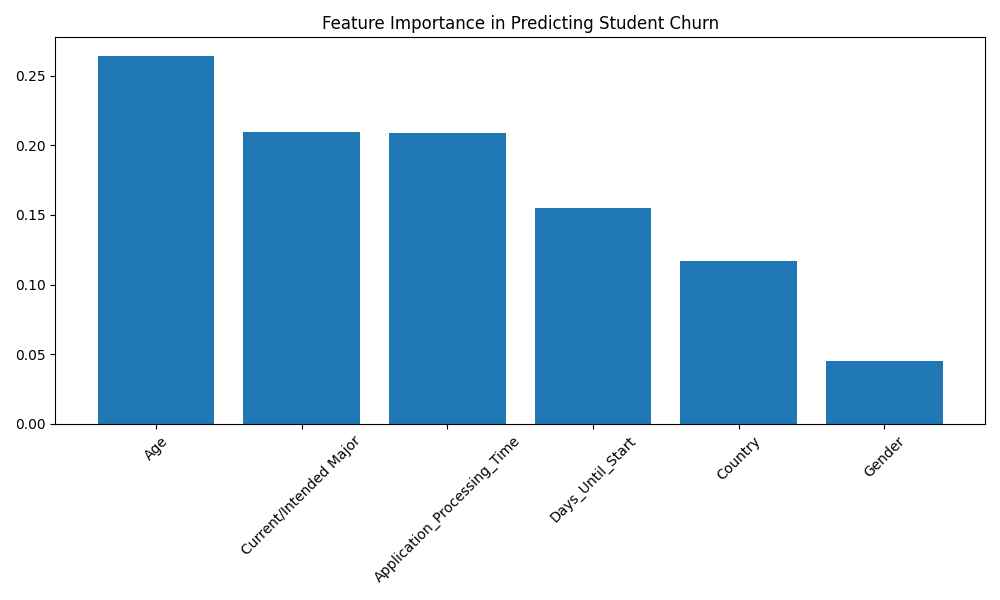
\includegraphics[width=0.8\textwidth]{../Code/images/feature_importance.png}
    \caption{Feature Importance Ranking}
    \label{fig:feature_importance}
\end{figure}

\begin{figure}[ht]
    \centering
    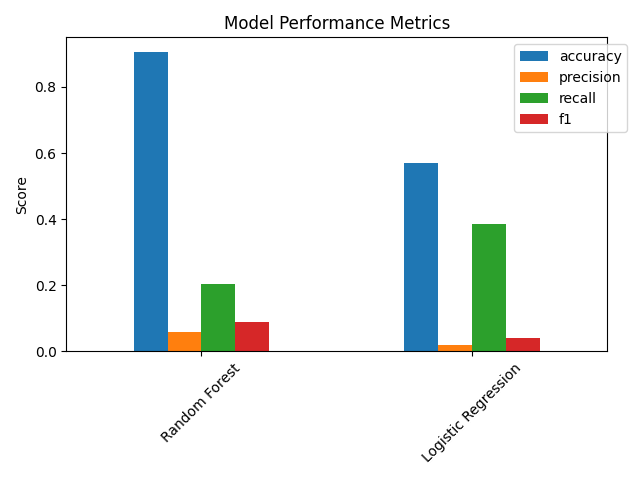
\includegraphics[width=0.8\textwidth]{../Code/images/model_metrics.png}
    \caption{Model Performance Metrics Comparison}
    \label{fig:model_metrics}
\end{figure}

\section{Recommendations}
Based on our analysis, we recommend:
\begin{enumerate}
    \item Early Intervention Program
    \begin{itemize}
        \item Monitor student engagement patterns
        \item Provide additional support during critical periods
    \end{itemize}
    
    \item Process Improvements
    \begin{itemize}
        \item Streamline application processing
        \item Optimize program start timing
    \end{itemize}
    
    \item Support Systems
    \begin{itemize}
        \item Implement mentorship programs
        \item Provide targeted resources based on student background
    \end{itemize}
    
    \item Continuous Monitoring
    \begin{itemize}
        \item Regular assessment of retention metrics
        \item Feedback loop for intervention effectiveness
    \end{itemize}
\end{enumerate}

\section{Conclusion}
This analysis provides actionable insights for improving student retention. Implementing the recommended strategies while maintaining continuous monitoring and adjustment will help optimize student success rates.

\end{document}
